\documentclass[DM,authoryear,toc,lsstdraft]{lsstdoc}
\usepackage[nonumberlist,nogroupskip,toc,numberedsection=autolabel]{glossaries}

\input meta.tex

\title{LSST Auxiliary Telescope observation strategy}
\author{
A.~Guyonnet
}

\setDocRef{\lsstDocType-\lsstDocNum}
\date{\vcsDate}


\setDocAbstract{%
LSST Auxiliary Telescope (A.T.) will supplement the survey photometric calibration with realtime atmospheric transmission monitoring. The A.T. is equipped with a low resolution spectrometer that will record dispersed images from stable natural celestial as they progress across the sky and back-light the atmosphere.
This report presents a strategy to follow the atmospheric transparency variability at a few permil level from assimilating A.T. spectra with ancillary data. The dataset is used to feed a radiative transport simulation which delivers the atmospheric optical transmission.
}

\setDocChangeRecord{%
  \addtohist{\vcsRevision}{\vcsDate}{Unreleased draft.}{Guyonnet}
}

\begin{document}

\maketitle

\section*{Introduction}

This report describes the A.T. observation strategy to deliver a permil monitoring of the atmospheric transparency along the LSST line of sight. The method is to build a forward model of the atmospheric transmission from the determination of four parameters: the precipitable water Vaper (PWV), the Aerosol optical depth (AOD), the ozone column depth and the molecular scattering. Together, they fully constrain radiative transfer codes which have been shown to deliver reliable atmospheric transparency curves (Mayer and Kylling 2005, Obregon et al. 2015, Smette et al. 2015). 


The parameters can be simultaneously determined from the fit of a single calibrated A.T. exposure. In practice, permil spectro-photometry has not been demonstrated yet and the single exposure solution remains partly degenerated with the telescope throughput uncertainties. A strategy that overcomes this limitation is to combine A.T. spectroscopy with data from global assimilation systems \citep{2018SPIE10704E..20C}.

Global assimilation systems routinely record variability of atmospheric constituents that translate into sub-percent variability of the atmospheric throughput. The avalanche of data from earth science experiments has been organized in a comprehensive manner by the Modern-Era Retrospective Analysis for Research and Applications, version 2 (MERRA-2)\footnote{\url{https://disc.sci.gsfc.nasa.gov/datasets?page=1&keywords=MERRA-2}}. This is the assimilation of satellites data from space agencies (NASA, ESA, Taiwan) as well as other external probes such as AERONET, aircrafts and cruise ships onboard instrumentation. Since the project is central for climate research, it has been under strong scrutiny and benefits from extensive analysis of consistency of the observations and the performance of assimilation methods (Randles et al. 2017 and references therein).

MERRA-2 tables are most relevant with respect to the determination of the ozone column depth and the molecular scattering: Ozone is found to vary on large temporal and spatial scales which makes it a parameter that can be reliably extracted from the MERRA-2 tables. The molecular scattering is driven by the temperature and barometric profile: it can be retrieved with sufficient precision from the interpolation of MERRA-2 tables above the LSST site. The remaining parameters, the PWV and the AOD are both varying on such scales that they are best captured by A.T. spectra: PWV level can be determined along the line-of-sight from a single A.T. exposure, while AOD is deduced from the difference of a pair of exposures. 

The section 1 details the steps to extract all the parameters from the A.T. and MERRA-2.


\section{Determination of the parameters of the model}


$\textrm{O}_2$ absorption is not a free parameter of the model. Instead the measurement of its equivalent width (EW) can be used as an estimator for biases in the method.


\subsection{Precipitable Water Vapor}


The total precipitable water vapor (PWV) in a vertical column is measured in $kg/m^2$ (sometimes in $mm$).  Its temporal evolution is correlated with the temperature and barometric pressure profiles in the vicinity of the telescope. It can exhibit significant local variability, such that smooth variation and axis-symmetry approximations are not valid. It is therefore best monitored by real time observations.

PWV can be determined along the line of sight of a single exposure by the measurement of the H$_2$O equivalent width (EW) in the range 880\,nm to 990\,nm.  


\subsection{Ozone}


The Ozone column depth impacts atmospheric transparency curve in two distinct regions: the Huggins band, below 350 nm, and the Chappuis bands, between 500 nm and 700 nm.
MERRA-2 tables indicate that O$_3$ concentrations at CTIO follow both seasonal and circadian variations,the annual distribution being between $6.5  \times  10^{18}$\,molecules cm$^{-2}$ (240 Dobsons) and $8.6  \times  10^{18}$\,molecules cm$^{-2}$ (320 Dobsons), and the circadian amplitude being typically in a 10-20 Dobsons range. \cite{doi:10.1002/2013JD020914} estimates that the value is correct to $\approx$1 Dobsons on large space (continental) and time (monthes) scales. Local tests are sparse but evidence for an $\approx$5 Dobsons uncertainty are presented \footnote{\url{https://confluence.lsstcorp.org/display/DM/2018-08-06+Calibration+Products+Standup}}. Since the assimilation process is updated every six hours, the conservative approach will be to use an averaged overnight value. 


\subsection{Molecular scattering}


The optical depth for scattering processes (Rayleigh and Mie scattering) is proportional to airmass and varies as a function of wavelength. It can be parametrized in the following way :
\begin{equation}
\tau_R = \frac{X(h, \theta)}{ 2770\,\mathrm{g}/\mathrm{cm}^2} \left( \frac{400\,\mathrm{nm}}{\lambda} \right)^4
\end{equation}
where $X(h, \theta)$ is the air column depth as a function of height $h$ and scattering angle $\theta$.
Its impact on the atmospheric transmission is therefore a function of the barometric pressure profile. Analysis of the daily variation of air columns above Antofogasta \footnote{\url{https://confluence.lsstcorp.org/display/DM/2018-08-21+Calibration+Products+Standup}} shows that it is sufficient to input a single parameter, the local barometric pressure, to reliably inform LibRadTran molecular scattering. 


\subsection{Aerosol Optical Depth}


Given that the A.T. spectrum ($S$) of a star is the product of its spectral energy distribution (SED) by the telescope and atmopsheric throughout:
\begin{equation}
  S(\lambda, z, t) = SED(\lambda) \times T_{tel}(\lambda, t) \times T_{atmo}(\lambda, z, t) 
\end{equation}
By examining the same stable target at two different airmasses $z_1$, $z_2$ on a scale where a steady aerosol level is expected, we can relate $T_{atmo}^{z1}(\lambda)$ and $T_{atmo}^{z2}(\lambda)$ to the difference of the two spectra at two airmasses ($S_{z1}, S_{z1}$):
\begin{equation}
  \frac{S_{z1}(\lambda)}{S_{z2}(\lambda)}  =\frac{T_{atmo}^{z1}(\lambda)}{T_{atmo}^{z2}(\lambda)}.
  \label{obs}
\end{equation}
In addition, following equation 5 in \cite{2013A&A...549A...8B},
\begin{equation}
T_{atmo}^{z}(\lambda) = 10^{-0.4 K_{atmo}(\lambda, z)},
\end{equation}
in a region free of telluric lines,
\begin{equation}
K_{atmo}(\lambda, z) = z k_r + z k_A + z k_{O_3}
\end{equation}
where $k_r$ is the Rayleigh scattering, $k_A$ the aerosol scattering and $k_{O_3}$ is the ozone absorption. Assuming aerosols follow an inverse power law with wavelength:
\begin{equation}
k_{A}(\lambda) = \tau \lambda^{-\alpha}
\end{equation}
Equation \ref{obs} can then be rewritten as
\begin{equation}
  \frac{S_{z_1}(\lambda)}{S_{z_2}(\lambda)}  =\frac{10^{-0.4 z_1 (k_r(\lambda) + k_{o3}(\lambda))} \cdot 10^{-0.4 z_1 \tau \lambda^{-\alpha}} }{10^{-0.4 z_2 (k_r(\lambda) + k_{o3}(\lambda))} \cdot 10^{-0.4 z_2 \tau \lambda^{-\alpha}}}.  
\end{equation}
Using a radiative transfer simulation (without aerosols) of the two observations at two airmasses:
\begin{equation}
  \frac{\Big(S_{z_1}(\lambda)/(S_{z_2}(\lambda)\Big)}{\Big({T_{atmo}^{z_1}}_{sim}^{noA}(\lambda)/({T_{atmo}^{z_2}}_{sim}^{noA}(\lambda)\Big)}  = 10^{-0.4 (z_2 - z_1)\tau \lambda^{-\alpha}}
\end{equation}
where $\tau$ is the AOD, and $\alpha$, the Angstrom exponent are the two parameters to be adjusted on spectra in a time series. 



\section{Validation of the method}


The two pillars of the observation plan are the stabilities of both the light sources above the atmosphere as well as the detector on the ground. Steady sub-percent stability of both components should be demonstrated. The method to extract the atmospheric transmission in between the stars and the telescope can be evaluated twice from comparing synthetic photometry with photometry, both from the A.T. and the main telescope. On the other end, the assimilation of NASA MERRA-2 data can checked against local weather probes.

\subsection{Modern-Era Retrospective Analysis for Research and Applications, version 2 (MERRA-2)}

Assimilating NASA MERRA-2 data for astronomy is innovative and relies on the validity of the interpolation: the accuracy of the local integration of the ozone column depth has been verified in several instances \citep{doi:10.1175/JCLI-D-16-0609.1}. An uncertainty of $\sim 5$ Dobsons is expected, which translates into 1 mmmag/airmass for the ozone peak at 6000 Å. It can change overnight by 20 Dobsons \citep{2013A&A...549A...8B}.

The spatio-temporal interpolation of the barometric pressure and temperature profiles has been tested against measurements from weather balloons launched from Antofogasta Airport: using either dataset impacts the molecular scattering is below the 1‰ level. 

PWV and aerosols above the LSST site are exhibiting localized and abrupt spatio-temporal variability. Precipitable Water Vapor at Cerro Tololo International Observatory (Same altitude as the LSST site, 6km away) routinely varies by 1 mm in an hour,  which is a 1\% transmission variation at 900-nm (Li et al. 2014). Aerosol optical depth can vary by 0.01 on an hourly basis, which is a 1\% transmission at 500-nm ( Guyonnet, LSST-DESC calibration Workshop June 2018). In this context, the reliability of local interpolation from global data need to be assessed thoroughly. This can be done from combaning local probes with weather forecast algorithms. Successful use for astronomy of such predictive algorithm has already been demonstrated at La Palma Roque de los Muchachos Observatory (\citealt{2018MNRAS.477.5477P}). The same context of abrupt orography surrounding LSST site advocates for implementing such a mesoscale control. To do so, an interdisciplinary approach is proposed and contacts have been taken with researchers from Laboratoire Atmosphères, Milieux, Observations Spatiales (LATMOS - CNRS, also on LPNHE Campus) that are specialized in studying the fundamental physico-chemistry processes of terrestrial atmosphere in their connections with the surface.


The optimal approach is to combine on-site measurements for pressure, temperature,
and humidity from the ground layer and up to the altitude where the wind direction remains mostly constant and independent of the observation dates. Above, it is assumed that the influence of the local environment has diminished and that global assimilation system can be used. The profiles should be regridded and weighted in order to provide a smooth transition from one dataset to the other.



\section{Radiative transfer codes}

There are at least three different codes that are available :
\begin{itemize}
\item LibRadtran is a software package for radiative transfer calculations\footnote{\url{https://www.geosci-model-dev.net/9/1647/2016/gmd-9-1647-2016.pdf}}
that has been used in more than more than 400 publications\footnote{\url{http://www.libradtran}}.
\item Molecfit \footnote{\url{ftp://ftp.eso.org/pub/dfs/pipelines/skytools/molecfit/VLT-MAN-ESO-19550-5772_Molecfit_User_Manual.pdf}} is a general tool for telluric absorption correction (\url{https://arxiv.org/pdf/1501.07239.pdf}). It uses the radiative transfer code Line-By-Line Radiative Transfer Model (LNFL v3.1 / LBLRTMv12.8) which is widely used in atmospheric and climate research studies. It has been tested at Cerro Paranal by combining on-site measurements from the ESO meteo monitor and satellite data (algorithmic accuracy is $\approx$ 0.5\%).
\item Modtran.
\end{itemize}



\subsection{Nightly variability and impact on the transmission curve}


Analysis of MERRA-2 tables at LSST site for the past decade brings evidences for :
\begin{itemize}
\item A large (1mm/10km) east-west PWV gradient.
\item PWV and ozone follow circadian variations and
\item they are anti-correlated on an annual basis.
\item Large variations of AOD, PWV and O$_3$ can sometimes occur within a few hours timespan. 
\item O$_3$ and PWV gradients go along the same direction.
\end{itemize}


\section{Selected sources}


Star with known SED can be obtained either from STIS Calspec data or from theoretical models.
The software parts consists in matching an observation with it's target, convert the SED to photon units and downgrade the resolution to match observations. The tools have been developped by the Harvard team and organized into two Python classes ({\it SED}, {\it resolution}). Alternatively, the publicly available Python package {\it pysynphot} \footnote{\url{http://pysynphot.readthedocs.io/en/latest/spectrum.html\#pysynphot-spectrum}} provides similar capabilities.


Table \ref{fig:im2} indicates the standard stars that have been routinely monitored by the SNFactory collaboration since 2006.

\begin{figure}
\centering
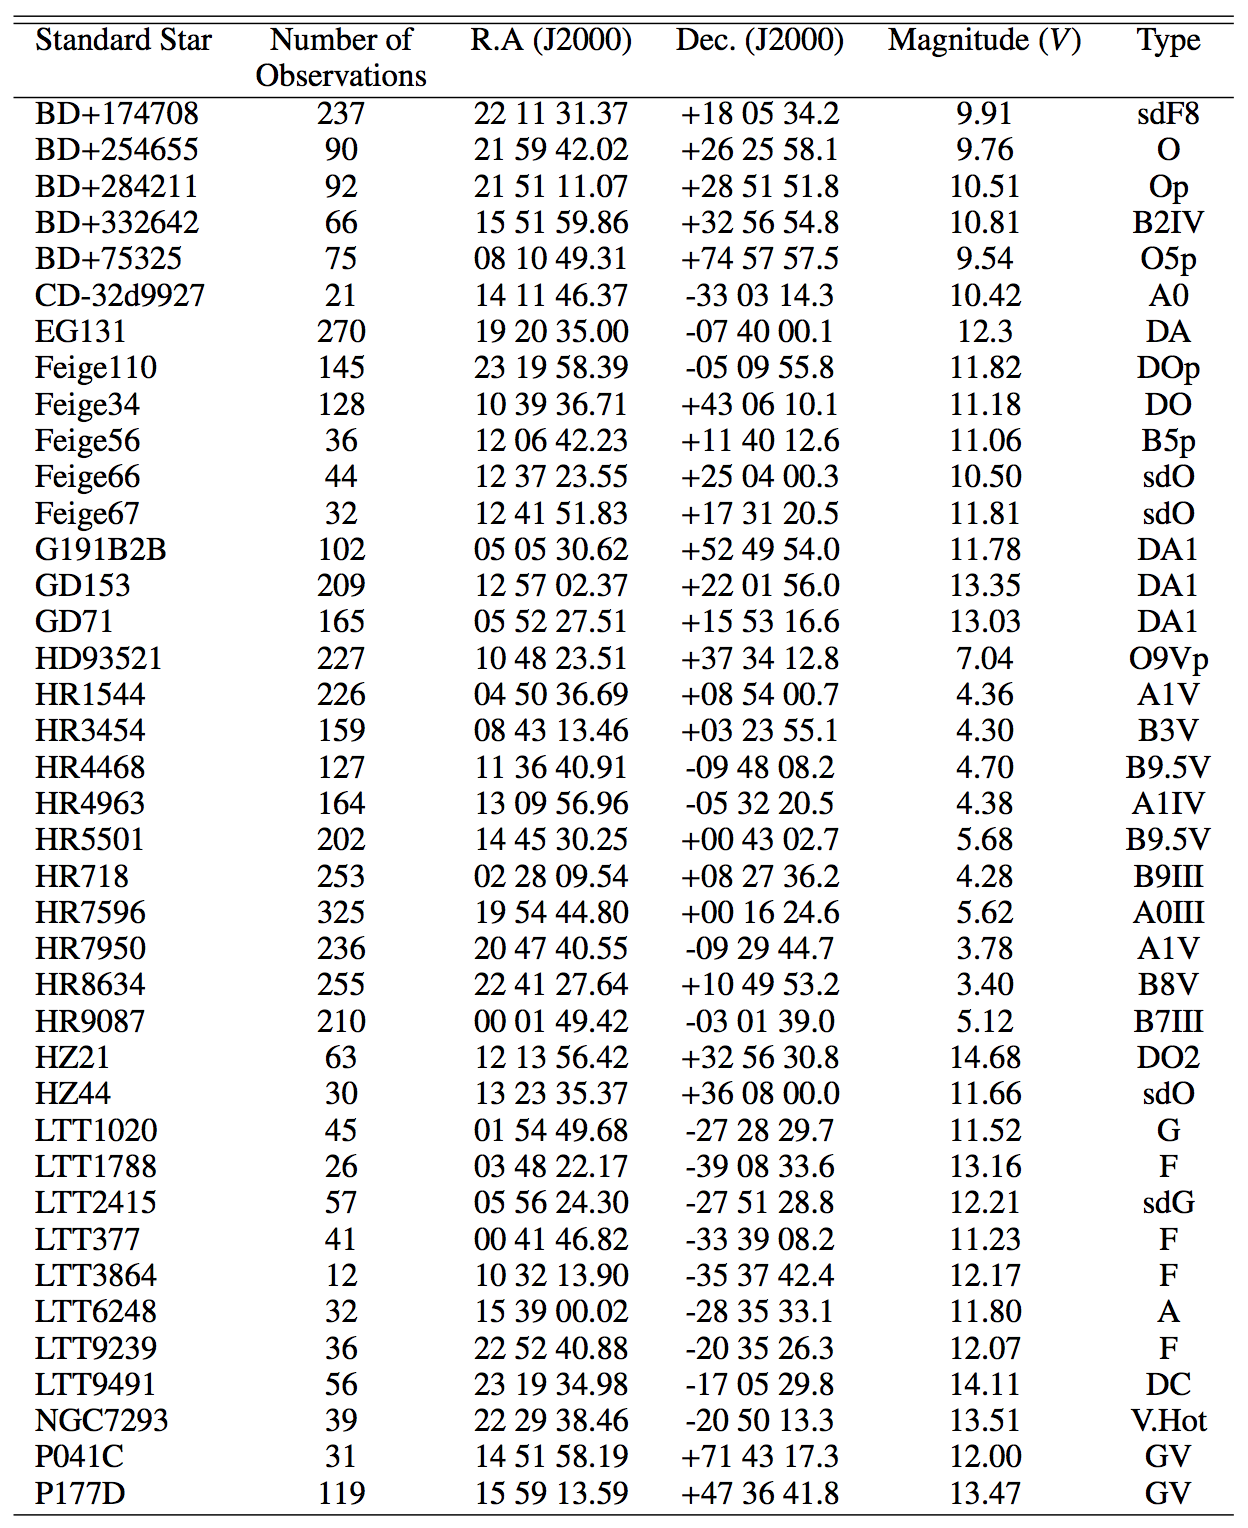
\includegraphics[width=0.6\linewidth]{figures/snf_target.png}
\caption{ List of the standard stars observed by the SNIF instrument mounted on the UH telescope and used by the SNfactory collaboration to monitor the atmospheric transmission \citep{2013A&A...549A...8B}.
\label{fig:im2}
}
\end{figure}

\bibliography{lsst,lsst-dm,refs_ads,refs,books}

\end{document}
